% Options for packages loaded elsewhere
\PassOptionsToPackage{unicode}{hyperref}
\PassOptionsToPackage{hyphens}{url}
%
\documentclass[
]{article}
\usepackage{amsmath,amssymb}
\usepackage{iftex}
\ifPDFTeX
  \usepackage[T1]{fontenc}
  \usepackage[utf8]{inputenc}
  \usepackage{textcomp} % provide euro and other symbols
\else % if luatex or xetex
  \usepackage{unicode-math} % this also loads fontspec
  \defaultfontfeatures{Scale=MatchLowercase}
  \defaultfontfeatures[\rmfamily]{Ligatures=TeX,Scale=1}
\fi
\usepackage{lmodern}
\ifPDFTeX\else
  % xetex/luatex font selection
\fi
% Use upquote if available, for straight quotes in verbatim environments
\IfFileExists{upquote.sty}{\usepackage{upquote}}{}
\IfFileExists{microtype.sty}{% use microtype if available
  \usepackage[]{microtype}
  \UseMicrotypeSet[protrusion]{basicmath} % disable protrusion for tt fonts
}{}
\makeatletter
\@ifundefined{KOMAClassName}{% if non-KOMA class
  \IfFileExists{parskip.sty}{%
    \usepackage{parskip}
  }{% else
    \setlength{\parindent}{0pt}
    \setlength{\parskip}{6pt plus 2pt minus 1pt}}
}{% if KOMA class
  \KOMAoptions{parskip=half}}
\makeatother
\usepackage{xcolor}
\usepackage[margin=1in]{geometry}
\usepackage{color}
\usepackage{fancyvrb}
\newcommand{\VerbBar}{|}
\newcommand{\VERB}{\Verb[commandchars=\\\{\}]}
\DefineVerbatimEnvironment{Highlighting}{Verbatim}{commandchars=\\\{\}}
% Add ',fontsize=\small' for more characters per line
\usepackage{framed}
\definecolor{shadecolor}{RGB}{248,248,248}
\newenvironment{Shaded}{\begin{snugshade}}{\end{snugshade}}
\newcommand{\AlertTok}[1]{\textcolor[rgb]{0.94,0.16,0.16}{#1}}
\newcommand{\AnnotationTok}[1]{\textcolor[rgb]{0.56,0.35,0.01}{\textbf{\textit{#1}}}}
\newcommand{\AttributeTok}[1]{\textcolor[rgb]{0.13,0.29,0.53}{#1}}
\newcommand{\BaseNTok}[1]{\textcolor[rgb]{0.00,0.00,0.81}{#1}}
\newcommand{\BuiltInTok}[1]{#1}
\newcommand{\CharTok}[1]{\textcolor[rgb]{0.31,0.60,0.02}{#1}}
\newcommand{\CommentTok}[1]{\textcolor[rgb]{0.56,0.35,0.01}{\textit{#1}}}
\newcommand{\CommentVarTok}[1]{\textcolor[rgb]{0.56,0.35,0.01}{\textbf{\textit{#1}}}}
\newcommand{\ConstantTok}[1]{\textcolor[rgb]{0.56,0.35,0.01}{#1}}
\newcommand{\ControlFlowTok}[1]{\textcolor[rgb]{0.13,0.29,0.53}{\textbf{#1}}}
\newcommand{\DataTypeTok}[1]{\textcolor[rgb]{0.13,0.29,0.53}{#1}}
\newcommand{\DecValTok}[1]{\textcolor[rgb]{0.00,0.00,0.81}{#1}}
\newcommand{\DocumentationTok}[1]{\textcolor[rgb]{0.56,0.35,0.01}{\textbf{\textit{#1}}}}
\newcommand{\ErrorTok}[1]{\textcolor[rgb]{0.64,0.00,0.00}{\textbf{#1}}}
\newcommand{\ExtensionTok}[1]{#1}
\newcommand{\FloatTok}[1]{\textcolor[rgb]{0.00,0.00,0.81}{#1}}
\newcommand{\FunctionTok}[1]{\textcolor[rgb]{0.13,0.29,0.53}{\textbf{#1}}}
\newcommand{\ImportTok}[1]{#1}
\newcommand{\InformationTok}[1]{\textcolor[rgb]{0.56,0.35,0.01}{\textbf{\textit{#1}}}}
\newcommand{\KeywordTok}[1]{\textcolor[rgb]{0.13,0.29,0.53}{\textbf{#1}}}
\newcommand{\NormalTok}[1]{#1}
\newcommand{\OperatorTok}[1]{\textcolor[rgb]{0.81,0.36,0.00}{\textbf{#1}}}
\newcommand{\OtherTok}[1]{\textcolor[rgb]{0.56,0.35,0.01}{#1}}
\newcommand{\PreprocessorTok}[1]{\textcolor[rgb]{0.56,0.35,0.01}{\textit{#1}}}
\newcommand{\RegionMarkerTok}[1]{#1}
\newcommand{\SpecialCharTok}[1]{\textcolor[rgb]{0.81,0.36,0.00}{\textbf{#1}}}
\newcommand{\SpecialStringTok}[1]{\textcolor[rgb]{0.31,0.60,0.02}{#1}}
\newcommand{\StringTok}[1]{\textcolor[rgb]{0.31,0.60,0.02}{#1}}
\newcommand{\VariableTok}[1]{\textcolor[rgb]{0.00,0.00,0.00}{#1}}
\newcommand{\VerbatimStringTok}[1]{\textcolor[rgb]{0.31,0.60,0.02}{#1}}
\newcommand{\WarningTok}[1]{\textcolor[rgb]{0.56,0.35,0.01}{\textbf{\textit{#1}}}}
\usepackage{graphicx}
\makeatletter
\def\maxwidth{\ifdim\Gin@nat@width>\linewidth\linewidth\else\Gin@nat@width\fi}
\def\maxheight{\ifdim\Gin@nat@height>\textheight\textheight\else\Gin@nat@height\fi}
\makeatother
% Scale images if necessary, so that they will not overflow the page
% margins by default, and it is still possible to overwrite the defaults
% using explicit options in \includegraphics[width, height, ...]{}
\setkeys{Gin}{width=\maxwidth,height=\maxheight,keepaspectratio}
% Set default figure placement to htbp
\makeatletter
\def\fps@figure{htbp}
\makeatother
\ifLuaTeX
  \usepackage{luacolor}
  \usepackage[soul]{lua-ul}
\else
  \usepackage{soul}
\fi
\setlength{\emergencystretch}{3em} % prevent overfull lines
\providecommand{\tightlist}{%
  \setlength{\itemsep}{0pt}\setlength{\parskip}{0pt}}
\setcounter{secnumdepth}{-\maxdimen} % remove section numbering
\usepackage{amsmath}
\usepackage{sectsty} \allsectionsfont{\centering}
\usepackage{booktabs}
\usepackage{longtable}
\usepackage{array}
\usepackage{multirow}
\usepackage{wrapfig}
\usepackage{float}
\usepackage{colortbl}
\usepackage{pdflscape}
\usepackage{tabu}
\usepackage{threeparttable}
\usepackage{threeparttablex}
\usepackage[normalem]{ulem}
\usepackage{makecell}
\usepackage{xcolor}
\ifLuaTeX
  \usepackage{selnolig}  % disable illegal ligatures
\fi
\usepackage{bookmark}
\IfFileExists{xurl.sty}{\usepackage{xurl}}{} % add URL line breaks if available
\urlstyle{same}
\hypersetup{
  pdfauthor={Nathan A. Nguyen},
  hidelinks,
  pdfcreator={LaTeX via pandoc}}

\title{\vspace{5cm}

GIS 563

Local Statistical Modeling

Final Project}
\author{Nathan A. Nguyen}
\date{10 December 2024}

\begin{document}
\maketitle

\newpage

\section{\texorpdfstring{\ul{Introduction}}{Introduction}}\label{introduction}

This write-up serves as the second part submission for the final project
in the class.

For this project, an empirical application of MGWR was performed and
compared with a global OLS model. The response variable was the
estimated median household income in 2021, and the spatial units were
United States counties. Details about the dataset and any preprocessing
that occurred will be discussed. The methods section will cover the
models explored and the software implementation as well as what R
packages were used for mapping for those who are interested. Finally
this write-up will close with brief discussions of the results and any
room for improvements should this be a real academic project.

The model presented in this write-up will deviate slightly from the
model presented in part 1. The modifications were made to accommodate
critiques while presenting -- namely the use of poverty level as a
predictor. This variable was replaced with the percentage of the
population in a respective county that are considered in an urban area.
During the initial presentation, the Monte Carlo test was still running,
so no results were available.

Due to time constraints, and unexpected events, a Monte Carlo test for
the existence of spatial variability was not performed. The Monte Carlo
test for the first version of this model did complete eventually, and it
suggested that the only variable with evidence for spatial variability
was the all age poverty levels in 2021. I included this variable
initially because although poverty is obviously associated with income,
I wanted to see whether or not the effects of poverty on median income
were uniform across space or if they changed based on geography.

That being said, a rigorous test for spatial variance will not be
provided for this second model presented.

\newpage

\section{\texorpdfstring{\ul{Data
Details}}{Data Details}}\label{data-details}

The dataset used for analysis is an amalgamation of various datasets
from the United States Census Bureau/United States Department of
Commerce, the American Community Survey, the United States Department of
Agriculture's Economic Research Service, and from a 2022 paper by
Fotheringham et al.,\textsuperscript{1} .

The area of study were United States counties, and only mainland
counties were intended to be retained in the dataset. For transparency,
most of Connecticut is missing and this issue was not observed until
after-the-fact. The missingness is attributed to the non-standardization
of FIP codes among the various datasets used. Some locations in
Connecticut are not considered true counties and are ``county
equivalents'', which was not known a-priori.

After preprocessing, the final dataset consisted of 3,100 locations.
Some R functions were defined in order to assist the preprocessing step
-- namely cleaning of FIP codes.

The chosen response variable was the estimated median household income
in the year 2021 and was provided by the Census Bureau/Department of
Commerce\textsuperscript{6}. Nine predictors were included in the
models:

\begin{enumerate}
\def\labelenumi{\arabic{enumi}.}
\item
  Gini Index (1-year estimate; 2021)\textsuperscript{5}
\item
  Population Density (natural logged)\textsuperscript{1}
\item
  Percent of Households with Internet Access (5-year estimate;
  2017-2022)\textsuperscript{2}
\item
  Percent of Population with Bachelors Degree or
  Higher\textsuperscript{3}
\item
  Percent of Population Living in an Urban Area(1-year estimate;
  2020)\textsuperscript{6}
\item
  Sex Ratio (Male-to-Female) (5-year estimate;
  2017-2022)\textsuperscript{4}
\item
  Median Age (5-year estimate; 2017-2022)\textsuperscript{4}
\item
  Percent Population that is Black (5-year estimate;
  2017-2022)\textsuperscript{4}
\item
  Percent Population that is Hispanic or Latino (5-year estimate;
  2017-2022)\textsuperscript{4}
\end{enumerate}

\begin{longtable}[t]{lcccc}
\caption{\label{tab:unnamed-chunk-2}Summary Statistics for Selected Variables}\\
\toprule
Variable & Min & Mean & Median & Max\\
\midrule
Median Income (21) & 25653.00 & 58741.99 & 56465.50 & 153716.00\\
Gini Index (17-21) & 0.25 & 0.45 & 0.44 & 0.73\\
Population Density (Natural Log) & -1.93 & 3.78 & 3.78 & 10.77\\
\% Internet Access (21) & 35.97 & 82.78 & 83.89 & 100.00\\
\% with Bachelor's Degree or Higher (18–22) & 0.00 & 23.44 & 20.90 & 78.90\\
\addlinespace
\% Population in Urban Area (20) & 0.00 & 35.95 & 33.41 & 100.00\\
Sex Ratio (Male:Female, 17–21) & 76.90 & 101.93 & 99.60 & 221.30\\
Median Age (17–21) & 22.40 & 41.52 & 41.30 & 68.10\\
\% Black (17–21) & 0.00 & 9.03 & 2.26 & 87.12\\
\% Hispanic or Latino (17–21) & 0.00 & 9.82 & 4.49 & 98.22\\
\bottomrule
\end{longtable}

\newpage

\begin{figure}[H]

{\centering \includegraphics[width=1\linewidth]{images/median-income21} 

}

\caption{Estimated Median Household Income (2021)}\label{fig:unnamed-chunk-3}
\end{figure}

Figure 1 shows the estimated median household income in 2021. By
inspection, there appears to be some clustering of this random variable.
For example, we see that the median household income is generally higher
in the north-east coast of the United States, indicated by the darker
coloring, when compared to the deep south and Appalachia, indicated by
the lighter shading. The west coast, generally, has higher income as
well.

This is likely due to the fact that the north-east and west-coast are
more developed regions of the country with high paying industries like
finance and technology while the regions with lower income are more
rural and have declining industries e.g., manufacturing and mining.

\newpage

Furthermore, the regions with higher median household income generally
have higher educational attainment as well. Figure 2 is evidence of
this:

\begin{figure}[H]

{\centering \includegraphics[width=1\linewidth]{images/bach-higher-18-22} 

}

\caption{Percent of Population Having Bachelors Degree or Higher}\label{fig:unnamed-chunk-4}
\end{figure}

\newpage

\section{\texorpdfstring{\ul{Methods}}{Methods}}\label{methods}

A global OLS and MGWR model was fit on the dataset and compared to one
another. The variance explained in both models were compared as well as
the AICc. All variables were standardized to have mean zero and and
variance one. Standardization was performed in R.

Ad-hoc tests were used in place of a Monte Carlo test:\\

\[
\begin{aligned}
IQR_{k} &> 2\times SE_{k-global}
\end{aligned}
\]

Corrected \(\alpha\)-values were computed following:

\[
\begin{aligned}
\alpha_{j} &= \frac{\alpha^{*}}{ENP_{j}}
\end{aligned}
\]

where \(\alpha^{*} = 0.05\) and the \(ENP_{j}\) were obtained from the
\texttt{txt} file from the MGWR 2.2 session.

\subsection{\texorpdfstring{\ul{Global OLS
Model}}{Global OLS Model}}\label{global-ols-model}

All features in the model are of order one, and no interaction terms
were considered.

\begin{table}[H]
\renewcommand{\arraystretch}{1.5} % Adjust row spacing
\centering
\caption{Global OLS Results}
\label{tab:ols_results}
\begin{tabular}{lcccc}
\hline
\textbf{Variable} & \textbf{Estimate} & \textbf{Std. Error} & \textbf{t-value} & \textbf{p-value} \\ \hline
Intercept             & 5.87e-17       & 1.00e-02         & 0.000             & 1.000 \\ 
Gini Index (17–21)    & -0.259         & 0.011            & -22.595           & $<$2e-16 *** \\ 
Population Density (Log) & 0.179         & 0.016            & 11.468           & $<$2e-16 *** \\ 
\% Internet Access (21)  & 0.237         & 0.015            & 15.627           & $<$2e-16 *** \\ 
\% Bachelor's Degree or Higher (18–22) & 0.579 & 0.014   & 41.660           & $<$2e-16 *** \\ 
\% Population in Urban Area (20) & -0.124 & 0.018        & -6.994           & 3.26e-12 *** \\ 
Sex Ratio (Male:Female, 17–21) & 0.351   & 0.107          & 3.295            & 0.000997 *** \\ 
Median Age (17–21)     & 0.099         & 0.118            & 0.845            & 0.398 \\ 
\% Black (17–21)       & -0.059        & 0.012            & -4.929           & 8.70e-07 *** \\ 
\% Hispanic or Latino (17–21) & 0.080    & 0.012          & 6.975            & 3.73e-12 *** \\ 
\hline
\multicolumn{5}{l}{\textit{Residual Standard Error:} 0.5578 on 3090 degrees of freedom} \\
\multicolumn{5}{l}{\textit{Multiple R-squared:} 0.6897, \textit{Adjusted R-squared:} 0.6888} \\
\multicolumn{5}{l}{\textit{F-statistic:} 763.3 on 9 and 3090 DF, \textit{p-value:} $<$2.2e-16} \\
\hline
\multicolumn{5}{l}{\textbf{Signif. Codes:} *** $p < 0.001$, ** $p < 0.01$, * $p < 0.05$} \\
\end{tabular}
\end{table}

According to the global model, all variables are statistically
significant at the level of \(0.05\) except for the median age variable.
Furthermore, the model is able to explain about \(69\%\) of the variance
in the data (adjusted and non-adjusted \(R^{2}\)). Despite these,
seemingly, good indicators, I'm skeptical about the usefulness of the
model. With sufficiently large sample sizes, any trivial relationship is
``statistically significant'', and other methods for evaluations should
be considered e.g., k-fold cross-validation, re-sampling methods, etc.
Alternatively, looking at the effect sizes and confidence intervals of
the parameter estimates might be more relevant to determine how ``good''
a model is, but this is likely domain specific, and so I have no further
comments on this.

A summary of the global OLS model results is contained in table 2. The
global model is able to explain approximately \(69\%\) of the variance
of standardized median income (adjusted \(R^{2}\)). Among all
predictors, all are statistically significant at \(\alpha = 0.05\)
except for median age.

Although the global model has strong explanatory power
(\(R_{adj}^{2} \approx 69\%\)), it is not without limitations. The
diagnostic plots (Figure 4) indicate potential violations in the
assumptions of linear regression -- name heteroskedasticity
(non-constant variance) and the distribution of the residuals being
non-normal. Figure 4 is evidence of heteroskedasticity as there is a
cone structure in the residuals. The residuals get larger for larger
predicted values of \(Y\). Furthermore, it can be observed that the
distribution of residuals has fatter right-tails and skinnier-left
tails. If the residuals were distributed normally, then the standardized
residuals would be more symmetric and it would hug the theoretical line
more tightly.

Figure 5 also suggests that higher-order terms, or at least some
transformation on the raw variables, might be necessary. The
component-residual plot for the percent with internet access variable
shows curvature in the data. This indicates a non-linear specification
of this variable might be the proper functional form. All other graphs
are relatively linear.

\begin{figure}[H]

{\centering 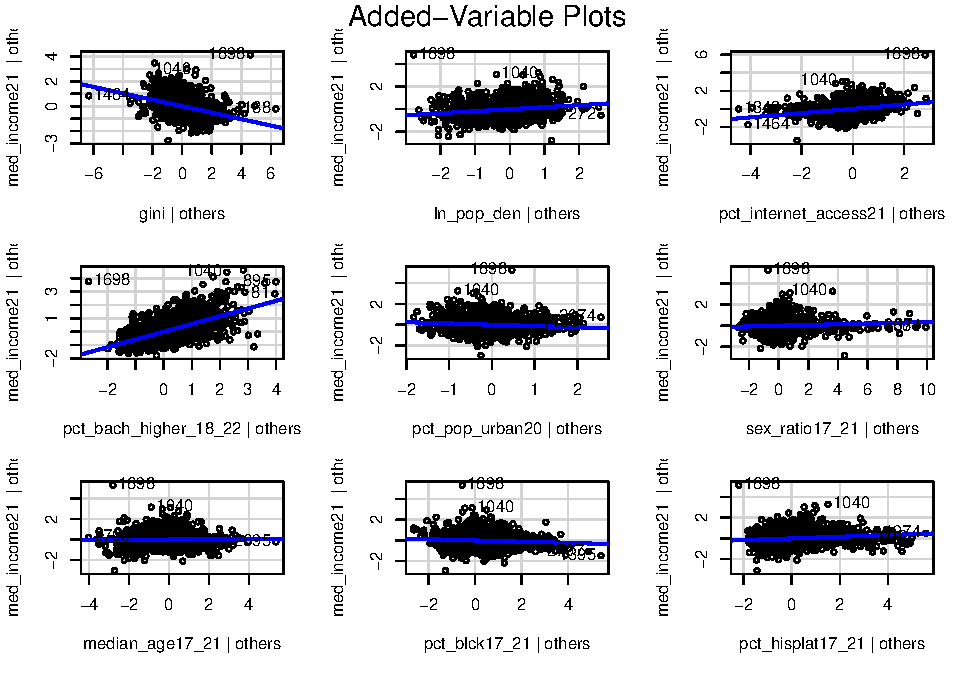
\includegraphics[width=1\linewidth]{final-project-write-up-nathan-nguyen_files/figure-latex/unnamed-chunk-6-1} 

}

\caption{Global OLS Added Variable Plots}\label{fig:unnamed-chunk-6}
\end{figure}

\newpage

The standardized \(\beta\)s represent the expected change in the
response variable \(Y\) (in standard deviations) for a one standard
deviation increase/decrease in some \(k^{th}\) predictor variable while
holding the other \(k-1\) variables constant.

The positive, and significant, set of coefficients is:

\(\{\text{Population Density, Internet Access, Bachelors Degree or Higher, Sex Ratio, Percent Hispanic or Latino}\}\)

For example, a one standard deviation increase in the percentage of the
population with a bachelor's degree or higher is associated with a 0.58
standard deviation increase in the expected standardized median income,
holding all other variables constant. This finding underscores the
critical role of higher education in driving income levels and aligns
with contemporary socioeconomic theories.

Furthermore, among the set of positive and significant predictors,
having a bachelors degree or higher has the largest absolute magnitude,
suggesting that if we had a homogeneous population, education attainment
might be the most important factor in one's possible earnings. This
conclusion makes sense because careers that, generally, pay more are
more technical and require at least a bachelors degree to obtain e.g.,
software engineering, banking, and so on.

On the other hand, the set of negative and significant coefficients is:

\(\{\text{Gini Index, Percent of Population Living in Urban Area, Percent Population that is Black}\}\)

The predictor having the most negative effect is the Gini Index (income
inequality). A one standard deviation increase in the Gini Index will
result in a 0.26 standard deviation decrease in the expected
standardized median income, holding all other variables constant. This
is a logical conclusion given that if the location has high income
inequality, then it would follow that the median income be lower as
there is a larger spread between high income households and low income
households. Since the median is a robust measure of central tendency,
one would observe more households with smaller median incomes.

\newpage

\begin{figure}[H]

{\centering 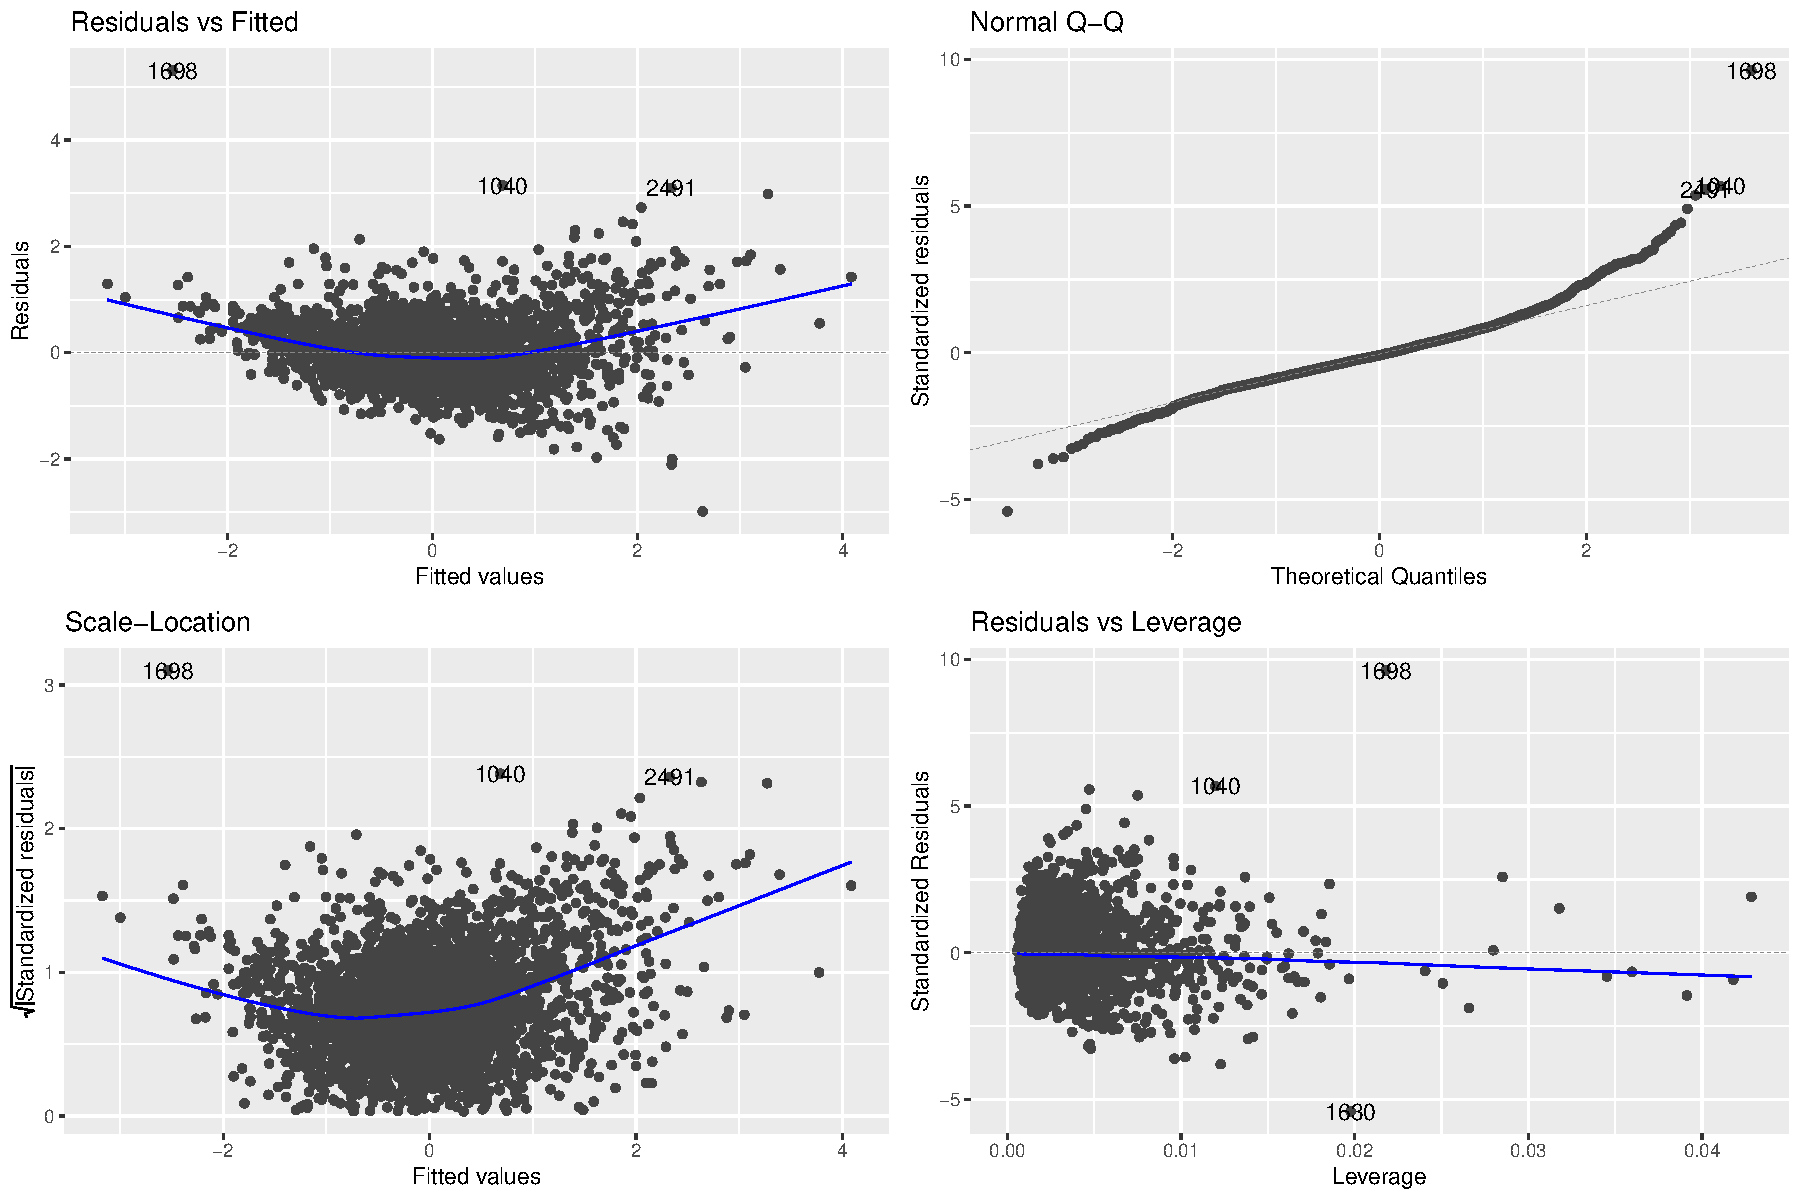
\includegraphics{final-project-write-up-nathan-nguyen_files/figure-latex/unnamed-chunk-7-1} 

}

\caption{Global OLS Diagnostics}\label{fig:unnamed-chunk-7}
\end{figure}

Figure 3 contains various diagnostic plots for the global OLS model.
Based on the residuals vs.~fitted values plot, the assumption of
constant variance appears to be violated i.e., the existence of
heteroskedasticity is likely. This is observed by the funnel structure
in the residuals for larger predicted values of \(Y\). Additionally, the
QQ plot of the residuals suggests a departure from normality, which is a
key assumption in linear regression. The distribution of residuals has
heavy right tails and skinnier left tails. A normal distribution should
be roughly symmetric, and if the model was correctly specified, the
observed residuals would hug the theoretical line more tightly.

There are two possible scenarios:

\begin{enumerate}
\def\labelenumi{\arabic{enumi}.}
\item
  spatial autocorrelation
\item
  first-order and main effects are not enough
\end{enumerate}

\begin{table}[H]
\renewcommand{\arraystretch}{1.3} % Adjust row spacing
\setlength{\tabcolsep}{12pt} % Adjust column spacing for wider table
\centering
\caption{Global OLS Residual Moran's I Test Results}
\label{tab:global_ols_morans_i}
\makebox[\textwidth]{ % Makes the table span the entire text width
\begin{tabular}{lcc}
\hline
\textbf{Statistic} & \textbf{Value} \\ \hline
Moran's I Statistic       & 0.3087 \\ 
Expectation               & -0.0003 \\ 
Variance                  & 0.0001 \\ 
Standard Deviate          & 28.675 \\ 
\textit{p-value}          & $<$ 2.2e-16 \\ 
\hline
\textbf{Alternative Hypothesis} & Greater \\ 
\multicolumn{2}{l}{\textit{Notes:} Moran's I test under randomization.} \\
\hline
\end{tabular}
}
\end{table}

\begin{figure}[H]

{\centering 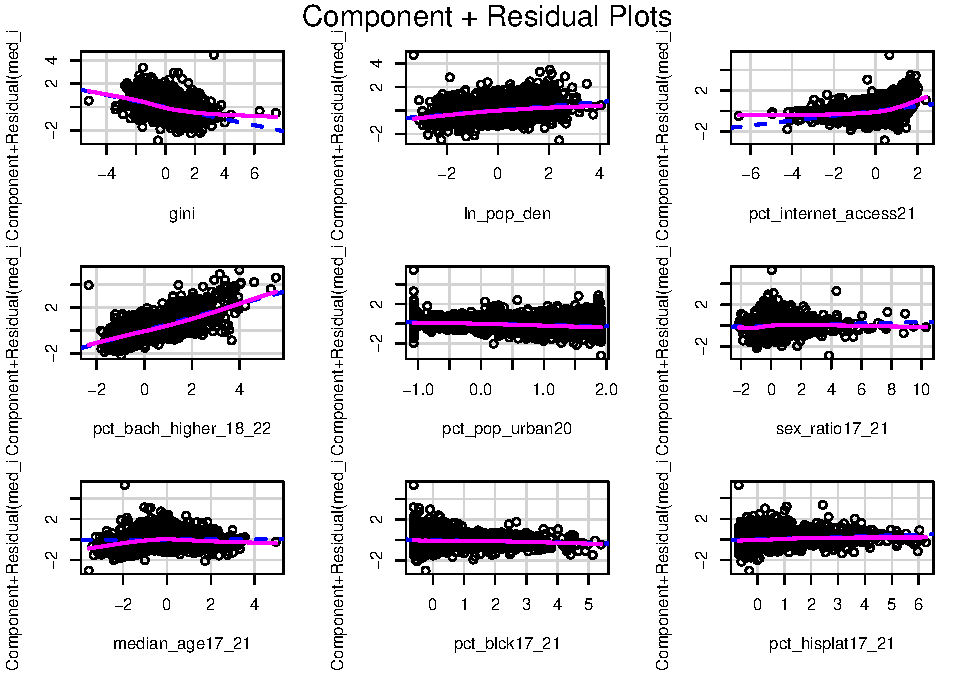
\includegraphics[width=1\linewidth]{final-project-write-up-nathan-nguyen_files/figure-latex/unnamed-chunk-9-1} 

}

\caption{Global OLS Component Regression Plots}\label{fig:unnamed-chunk-9}
\end{figure}

\newpage

\subsection{\texorpdfstring{\ul{MGWR
Model}}{MGWR Model}}\label{mgwr-model}

\begin{table}[H]
\renewcommand{\arraystretch}{1.3}
\centering
\caption{MGWR Model Summary}
\label{tab:mgwr_summary}
\begin{tabular}{lccccc}
\hline
\textbf{Variable} & \textbf{Min} & \textbf{Mean} & \textbf{Median} & \textbf{Max} & \textbf{Bandwidth (95\% CI)} \\ \hline
Intercept                & -0.584 & 0.007 & -0.018 & 0.949 & 44 [44, 44] \\ 
Gini Index (17–21)       & -0.568 & -0.206 & -0.193 & 0.055 & 92 [82, 107] \\ 
Population Density (Log) & -0.172 & 0.040 & 0.063 & 0.196 & 588 [488, 764] \\ 
\% Internet Access (21)  & -0.390 & 0.269 & 0.230 & 1.143 & 44 [44, 46] \\ 
\% Bachelor's Degree or Higher (18–22) & -0.137 & 0.471 & 0.477 & 0.971 & 52 [48, 57] \\ 
\% Population in Urban Area (20) & -0.071 & -0.049 & -0.050 & -0.028 & 2263 [1932, 2654] \\ 
Sex Ratio (Male:Female, 17–21) & -0.004 & 0.032 & 0.029 & 0.136 & 626 [488, 764] \\ 
Median Age (17–21)       & -0.297 & 0.041 & 0.060 & 0.258 & 142 [132, 172] \\ 
\% Black (2017–2021)     & -0.228 & -0.226 & -0.226 & -0.225 & 3098 [2378, 3098] \\ 
\% Hispanic or Latino (17–21) & -0.195 & 0.044 & 0.067 & 0.252 & 473 [423, 594] \\ \hline
\textbf{Metric} & \multicolumn{5}{l}{} \\ \hline
Residual Sum of Squares  & \multicolumn{5}{r}{328.055} \\
Log-Likelihood           & \multicolumn{5}{r}{-917.446} \\
AIC                      & \multicolumn{5}{r}{3023.785} \\
AICc                     & \multicolumn{5}{r}{3306.439} \\
BIC                      & \multicolumn{5}{r}{6613.743} \\
R\textsuperscript{2}     & \multicolumn{5}{r}{0.894} \\
Adjusted R\textsuperscript{2} & \multicolumn{5}{r}{0.869} \\
Degree of Dependency (DoD) & \multicolumn{5}{r}{0.492} \\ \hline
\end{tabular}
\end{table}

\begin{table}[H]
\renewcommand{\arraystretch}{1.3}
\centering
\caption{Comparison: Global OLS vs. MGWR}
\label{tab:ols_vs_mgwr}
\begin{tabular}{lcccc}
\hline
\textbf{Variable} & \textbf{OLS Estimate} & \textbf{MGWR Mean} & \textbf{MGWR Median} \\ \hline
Intercept                & 0.000 & 0.007 & -0.018 \\ 
Gini Index (17–21)       & -0.259 & -0.206 & -0.193 \\ 
Population Density (Log) & 0.179 & 0.040 & 0.063 \\ 
\% Internet Access (21)  & 0.237 & 0.269 & 0.230 \\ 
\% Bachelor's Degree or Higher (18–22) & 0.578 & 0.471 & 0.477 \\ 
\% Population in Urban Area (20) & -0.124 & -0.049 & -0.050 \\ 
Sex Ratio (Male:Female, 17–21) & 0.035 & 0.032 & 0.029 \\ 
Median Age (17–21)       & 0.010 & 0.041 & 0.060 \\ 
\% Black (2017–2021)     & -0.060 & -0.226 & -0.226 \\ 
\% Hispanic or Latino (17–21) & 0.080 & 0.044 & 0.067 \\ \hline
\textbf{Metric} & \textbf{Global OLS} & \textbf{MGWR} \\ \hline
Residual Sum of Squares  & 961.468 & 328.055 \\
Log-Likelihood           & -2584.131 & -917.446 \\
AIC                      & 5188.262 & 3023.785 \\
AICc                     & 5190.347 & 3306.439 \\
BIC                      & N/A & 6613.743 \\
R\textsuperscript{2}     & 0.690 & 0.894 \\
Adjusted R\textsuperscript{2} & 0.689 & 0.869 \\
Degree of Dependency (DoD) & N/A & 0.492 \\ \hline
\end{tabular}
\end{table}
\begin{table}[H]
\renewcommand{\arraystretch}{1.3} % Adjust row spacing
\setlength{\tabcolsep}{12pt} % Adjust column spacing for wider table
\centering
\caption{MGWR Residual Moran's I Test Results}
\label{tab:mgwr_morans_i}
\makebox[\textwidth]{ % Makes the table span the entire text width
\begin{tabular}{lcc}
\hline
\textbf{Statistic} & \textbf{Value} \\ \hline
Moran's I statistic       & 0.0023 \\ 
Expectation               & -0.0003 \\ 
Variance                  & 0.0001 \\ 
Standard Deviate          & 0.2432 \\ 
\textit{p-value}          & 0.4039 \\ 
\hline
\textbf{Alternative Hypothesis} & Greater \\ 
\multicolumn{2}{l}{\textit{Notes:} Moran's I test under randomization.} \\
\hline
\end{tabular}
}
\end{table}

\begin{figure}[H]

{\centering \includegraphics[width=1\linewidth]{images/nonlinearity/local-betas-vs-x} 

}

\caption{MGWR Diagnostic Plots}\label{fig:unnamed-chunk-10}
\end{figure}

\newpage

The effects of internet access are regional, given that the bandwidth is
essentially as large as the number of locations (3,100). Having access
to internet indicates higher median income likely an indication of more
developed localities.

The effects of having a bachelor's degree or higher are very local given
its small bandwidths and clustering observed in the map. Having more
education has a much stronger positive impact on one's median income in
Colorado, New Jersey, and some parts of Ohio wen compared to Arizona and
Idaho for example. It's also interesting to note the clustering in the
Appalachia area as well. Some pockets with higher education attainment
have higher income levels compared to neighbors in the area.

\newpage

\section{\texorpdfstring{\ul{Conclusions}}{Conclusions}}\label{conclusions}

\subsection{\texorpdfstring{\ul{Improvements}}{Improvements}}\label{improvements}

If I were to write a real paper on something like this, I'd probably
change my response variable to something that reflects discretionary
income more e.g., the median household income after adjusting for
housing costs. While people in California, New York, and Washington
might make a lot more than say, someone living in Alabama, people living
in California, New York, or Washington likely have a much larger housing
cost when compared to someone living in Alabama.

A transformation of some of the predictor variables might be warranted
given some non-linearity observed in both OLS and MGWR diagnostic plots.

Finally, a thorough literature review would have been beneficial in
order to understand the unique socioeconomic profiles of the US
counties. This would have aided in better understanding the results of
MGWR and/or helped validated existing theories in the literature. A
review would have also provided a better foundation for variable
selection in the models e.g., including employment industry variables,
and so on.

For those who are interesting in creating the maps in R, please refer to
my Github Repo:
\url{https://github.com/loafing-cat/gis563-local-stat-model-example}.

The following are the core R libraries for mapping:

\begin{Shaded}
\begin{Highlighting}[]
\FunctionTok{library}\NormalTok{(tidyverse)}
\FunctionTok{library}\NormalTok{(sf)}
\FunctionTok{library}\NormalTok{(tigris)}
\FunctionTok{library}\NormalTok{(colorspace)}
\end{Highlighting}
\end{Shaded}

\newpage

\section{\texorpdfstring{\ul{References}}{References}}\label{references}

\begin{enumerate}
\def\labelenumi{\arabic{enumi}.}
\item
  Li, Z., \& Fotheringham, A. S. (2022). The spatial and temporal
  dynamics of voter preference determinants in four U.S. presidential
  elections (2008-- 2020). Transactions in GIS, 26, 1609-- 628.
  \url{https://doi.org/10.1111/tgis.12880}
\item
  U.S. Census Bureau. (2022). Internet Subscriptions in Household.
  American Community Survey, ACS 5-Year Estimates Detailed Tables, Table
  B28011. Retrieved December 7, 2024, from
  \url{https://data.census.gov/table/ACSDT5Y2022.B28011?q=Telephone},
  Computer, and Internet Access\&g=010XX00US\$0500000.
\item
  United States Department of Agriculture, Economic Research Service.
  (2022). County-Level Data Sets: Poverty estimates. Retrieved from
  \url{https://www.ers.usda.gov/data-products/county-level-data-sets/county-level-data-sets-download-data/}
\item
  U.S. Census Bureau. (2021). ACS DEMOGRAPHIC AND HOUSING ESTIMATES.
  American Community Survey, ACS 5-Year Estimates Data Profiles, Table
  DP05. Retrieved December 9, 2024, from
  \url{https://data.census.gov/table/ACSDP5Y2021.DP05?q=Density&t=Populations}
  and People\&g=010XX00US\$0500000.
\item
  U.S. Census Bureau. (2021). GINI INDEX OF INCOME INEQUALITY. American
  Community Survey, ACS 5-Year Estimates Detailed Tables, Table B19083.
  Retrieved December 9, 2024, from
  \url{https://data.census.gov/table/ACSDT5Y2021.B19083?q=gini&g=010XX00US$0400000}.
\item
  United States Census Bureau. (2023). County-level 2020 Census Urban
  and Rural Information for the U.S., Puerto Rico, and Island Areas
  sorted by state and county FIPS codes {[}Data file{]}. Retrieved from
  \url{https://www.census.gov/programs-surveys/geography/guidance/geo-areas/urban-rural.html}
\end{enumerate}

\end{document}
